\section{Skin lesion classifier}
For the skin lesion competition I developed a model in collaboration with Marcus Hansen, Sarah Hansen and Ulrik Larsen. This model consists of six blocks of 3 by 3 convolutions with a ReLU activation function followed by a batch normalization followed by a 2 by 2 max pooling. For the convolutions padding with zeros have been used to keep the result after convolutions the same as the input size. After these six blocks, three blocks of a fully connected layer with a ReLU activation function followed by a batch normalization is used. The first fully connected layer has size 32, the second 16 and the last has 8. Lastly we have a fully connected layer of size 1 with a sigmoid activation function to get the class probability. This model has been trained with binary cross entropy as the loss function and an Adam optimizer with initial learning rate 0.00001. For the competition this model was trained for 1000 epochs using random affine transformations on the training data. The \textbf{final training accuracy} was around \textbf{0.90}, the \textbf{final validation accuracy} was around \textbf{0.80} and the \textbf{final test accuracy} was around \textbf{0.70}.\\
To evaluate this classification model I have been retraining the model, however, due to limitations in hardware I have only been able to train for 100 epochs. To compensate for this, I have used a learning rate of 0.0001 (a factor 10 larger) instead. The metrics I have chosen to use to evaluate the model are \textit{accuracy}, \textit{area under the ROC curve} and \textit{area under the precision / recall curve}. Accuracy simply tells us how many correctly classified images we got, i.e. true positives plus true negatives. Area under the ROC curve is given by measuring the area under the curve of a ROC curve. A ROC curve is made by plotting the sensitivity vs 1-specificity and tells us about the trade-off between the true positive rate and the false positive rate, i.e. the percentage of true positives we expect to find if we allow for some false positives. The area under the precision / recall curve is given by measuring the area under a precision / recall curve. Precision / recall curves measures how good the model is at predicting the positive class vs the ratio of true positives and false positives. Precision / recall curves can be relevant when we have imbalanced data, as the curve describes how often we predict true positive without introducing false negative, that is, we disregard the true negative 'accuracy'.

\begin{figure}
	\centering
	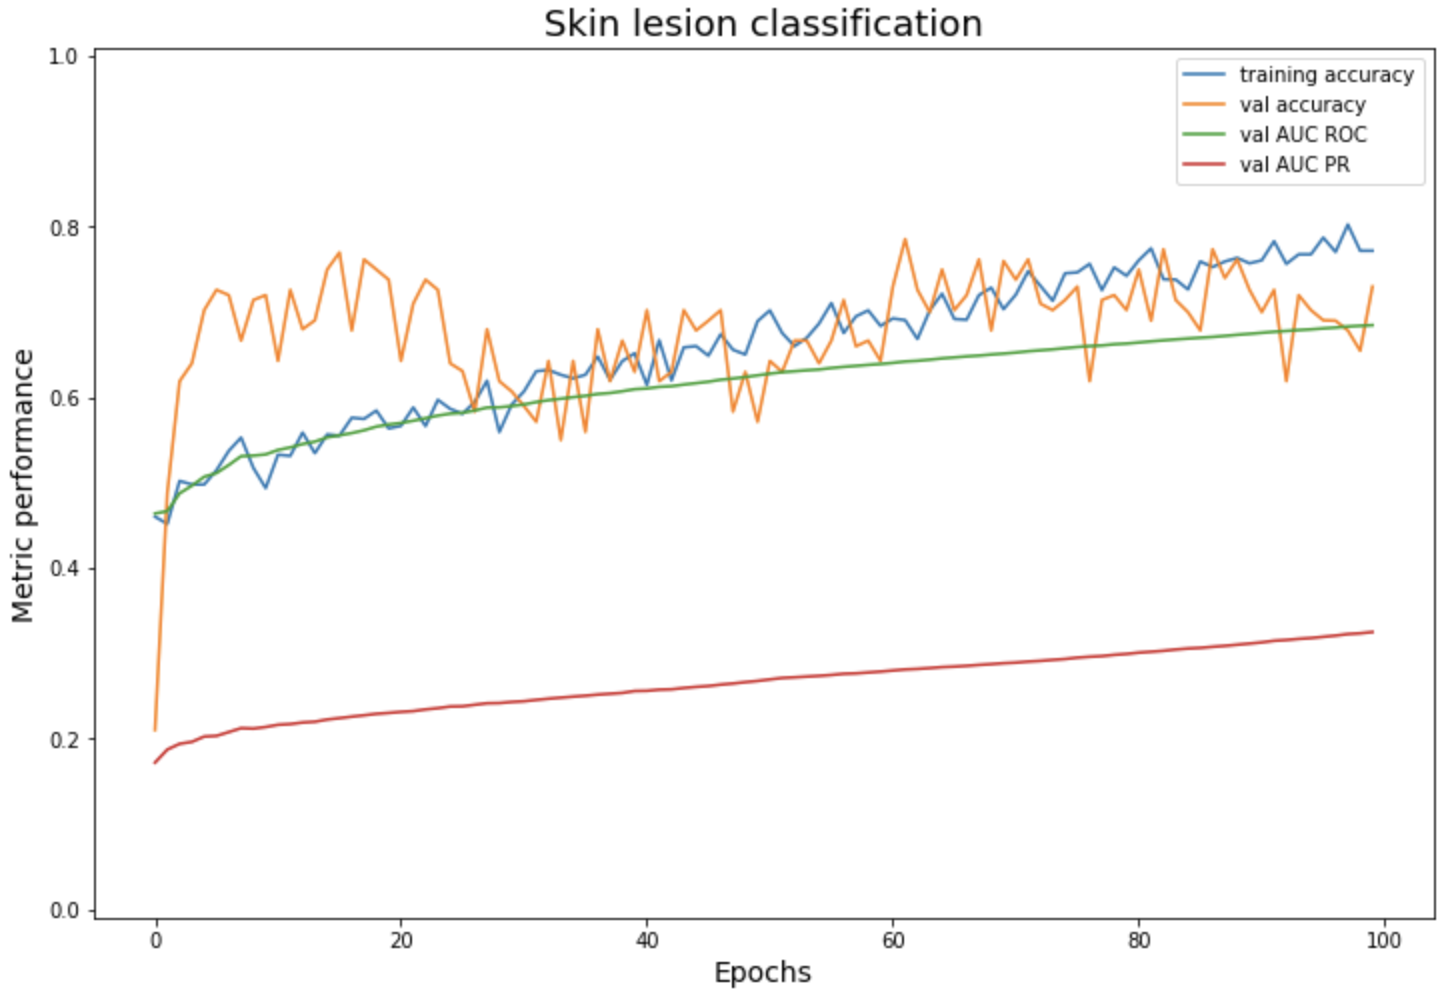
\includegraphics[width=0.88\linewidth]{Materials/skinlesion}
	\caption{Performance of the retrained skin lesion classifier.}
	\label{skinlesion}
\end{figure}
In \autoref{skinlesion} we see the training and validation accuracy along the area under the ROC curve and area under the precision / recall curve. We note these results are not as good as the results of the original model based on the validation accuracy. However, an accuracy of about 0.7 on unknown data is not ideal, but the model has learnt something. We note both the validation and training accuracy are still increasing and so, more epochs would probably have improved the model. When looking at area under the curve for ROC, we note it is steadily improving, which means we are getting better and better at predicting true positives without having to include more false positives. Lastly we note the area under the curve for precision / recall is also steadily increasing, which means we are getting better at predicting true positives without predicting false negatives. 